% !Mode:: "TeX:UTF-8"

\section{项目成果与反思}

\subsection{成果展示}
本项目成功设计并实现了一套基于STM32F103C8T6的智能手表系统，主要成果包括：

\subsubsection{硬件系统成果}
\begin{itemize}
    \item 完成基于STM32F103C8T6的最小系统搭建，成功驱动SSD1306 OLED、MPU6050六轴传感器、HC-05蓝牙三大外设
    \item 采用双路I2C总线设计（OLED使用I2C1，MPU6050使用I2C2），避免设备地址冲突和总线竞争
    \item 实现I2C总线恢复机制，解决从机死锁问题，系统启动成功率达100\%
    \item 系统在5V/1A供电下稳定工作，所有模块工作温度均在正常范围内（连续运行4小时无过热）
\end{itemize}

\subsubsection{固件软件成果}
\begin{itemize}
    \item 完成完整OLED显示驱动，支持三种尺寸字模显示和多页面UI（表盘/传感器/蓝牙/设备信息/活动计步）
    \item 实现MPU6050六轴数据采集与物理量转换，支持Pitch/Roll姿态角实时计算
    \item 设计自定义蓝牙帧协议（STX/CMD/DATA/CHK/ETX），含XOR校验，支持三种命令类型
    \item 实现基于加速度向量幅值+动态阈值的计步器算法，步行精度达97.5\%以上
    \item 实现TIM2驱动的软RTC时钟，支持蓝牙时间同步命令更新
    \item 采用DMA+空闲中断环形缓冲方案，蓝牙通信丢帧率降至0.15\%
    \item 固件总代码量约2000行C代码，模块化设计便于维护和扩展
\end{itemize}

\subsubsection{Android上位机成果}
\begin{itemize}
    \item 开发Material Design 3风格的Android APP，支持蓝牙设备扫描、连接管理
    \item 实现与手表端一致的帧协议解析器，正确解析传感器数据、时间同步、计步数据
    \item 提供实时传感器数据展示卡片、通信日志列表、时间同步按钮
    \item 深色/浅色主题切换，适配Android 8.0及以上版本（API 26+）
    \item APP总代码量约800行Kotlin代码，使用现代Android开发架构
\end{itemize}

\subsection{项目评估}

\subsubsection{成功之处}
\begin{itemize}
    \item \textbf{功能完整性：} 100\%实现了项目设计目标中的全部功能（OLED显示、六轴传感、蓝牙通信、计步算法、Android上位机）
    \item \textbf{系统稳定性：} 经过连续4小时以上的运行测试，系统无死机、无异常重启，I2C通信稳定，蓝牙连接可靠
    \item \textbf{通信协议设计：} 自定义的轻量级帧协议结构简单、扩展性好，XOR校验提供基本的数据完整性保护
    \item \textbf{计步算法精度：} 通过滤波、动态阈值、防抖等多重优化，步行精度达97.5\%（误差率$<$2.5\%），达到消费级智能手环基本水平
    \item \textbf{代码可维护性：} 模块化设计，每个功能模块独立（oled/mpu6050/bluetooth/pedometer/soft\_rtc等），接口清晰，便于后续扩展
    \item \textbf{成本控制：} 硬件总成本控制在100元以内，具有良好的性价比和推广潜力
    \item \textbf{Android端协同：} 手表-手机双向通信功能完整，数据展示和时间同步功能正常
\end{itemize}

\subsubsection{不足之处}
\begin{itemize}
    \item \textbf{用户交互局限：} 手表端无物理按键，OLED页面自动切换，用户无法主动选择显示内容
    \item \textbf{显示内容有限：} 128$\times$64单色OLED分辨率较低，无法显示更丰富的图形和中文内容
    \item \textbf{无数据持久化：} 步数、RTC时间等数据在断电后全部丢失，无Flash/EEPROM存储
    \item \textbf{蓝牙功耗偏高：} HC-05模块始终处于连接状态，未实现低功耗休眠模式，手表功耗约30mA，依赖USB供电
    \item \textbf{未实现手势识别：} MPU6050的陀螺仪数据仅用于姿态角显示，未充分利用于手势/动作识别
    \item \textbf{缺少专业传感器：} 无心率传感器、血氧传感器等健康监测必备组件，计步功能为唯一健康指标
    \item \textbf{机械结构简陋：} 基于面包板+杜邦线的原型方案，未实现封装，无法作为实际可穿戴设备使用
    \item \textbf{Android APP功能简单：} 仅实现基本数据展示，缺少历史数据统计、图表可视化、云同步等功能
\end{itemize}

\subsection{个人反思}

\subsubsection{理论与实践结合的收获}
\begin{itemize}
    \item \textbf{I2C通信协议：} 通过实际驱动OLED和MPU6050两个I2C设备，深入理解了START/STOP信号、ACK应答、读写时序等I2C协议核心机制，并通过I2C总线恢复的实现加深了对总线异常处理的理解
    \item \textbf{USART串口通信：} 通过实现HC-05蓝牙数据收发，掌握了波特率配置、数据位/停止位格式、DMA传输、空闲中断等串口通信高级特性
    \item \textbf{传感器数据处理：} 通过实现计步器算法，掌握了MEMS传感器数据的低通滤波、峰值检测、动态阈值等信号处理技术
    \item \textbf{中断驱动编程：} TIM2 1Hz中断、USART2 DMA空闲中断的实现，强化了中断上下文和主循环任务调度的理解
    \item \textbf{跨平台通信协议：} 自定义蓝牙帧协议的实现，锻炼了在嵌入式设备与Android应用之间设计统一通信格式的能力
\end{itemize}

\subsubsection{工程调试能力提升}
\begin{itemize}
    \item 学会了使用万用表测量电源电压、使用逻辑分析仪观察I2C波形
    \item 掌握了通过ST-Link进行JTAG/SWD调试、设置断点、观察寄存器状态的方法
    \item 学会了分模块调试：先验证OLED点亮，再接MPU6050，最后联调蓝牙，逐步递进
    \item 理解了软硬件协同调试思路，例如在DMA环形缓冲中设置调试标志位追踪问题
\end{itemize}

\subsubsection{项目管理与团队协作}
\begin{itemize}
    \item 学会了将一个完整项目拆分为硬件选型、固件开发、APP开发、集成测试等阶段
    \item 与队友方旭亮（硬件调试）和陈斯焕（Android UI）进行了有效分工配合
    \item 认识到文档和注释的重要性，在代码中添加了完整的功能说明
\end{itemize}

\subsection{改进方向}
针对项目不足之处，未来可从以下方面进行改进和扩展：

\begin{enumerate}
    \item \textbf{增加用户按键交互：} 添加1-2个物理按键或电容触摸按键，支持用户手动切换页面、重置计步、触发时间同步
    \item \textbf{使用更大屏幕OLED或TFT：} 更换为1.3寸240$\times$240彩色TFT显示屏，支持显示更丰富的UI和图形
    \item \textbf{添加数据持久化存储：} 使用STM32内部Flash或外挂EEPROM存储步数、时间等数据，支持断电恢复
    \item \textbf{实现蓝牙低功耗模式：} 添加HC-05休眠/唤醒逻辑，或更换为低功耗BLE模块（如Nordic nRF52832）
    \item \textbf{增加手势识别功能：} 利用MPU6050六轴数据实现抬手亮屏、翻腕切页等智能手表常见手势
    \item \textbf{添加健康监测传感器：} 扩展MAX30102心率/血氧传感器模块，升级为真正的健康监测设备
    \item \textbf{设计PCB外壳：} 将面包板原型升级为专业PCB板，设计3D打印外壳，实现可穿戴形态
    \item \textbf{增强Android APP功能：} 添加历史数据图表（使用MPAndroidChart库）、用户设置、云端同步（Firebase）
    \item \textbf{支持固件OTA升级：} 设计蓝牙OTA升级协议，支持通过手机无线更新手表固件
    \item \textbf{加入温湿度/气压传感：} 扩展BME280等环境传感器，实现天气监测功能
    \item \textbf{实现闹钟/定时器功能：} 基于软RTC实现闹钟提醒，配合蜂鸣器
    \item \textbf{电源管理优化：} 使用锂电池供电+TP4056充电模块，实现真正的移动可穿戴设备
\end{enumerate}

\FloatBarrier
\begin{figure}[h]
    \centering
    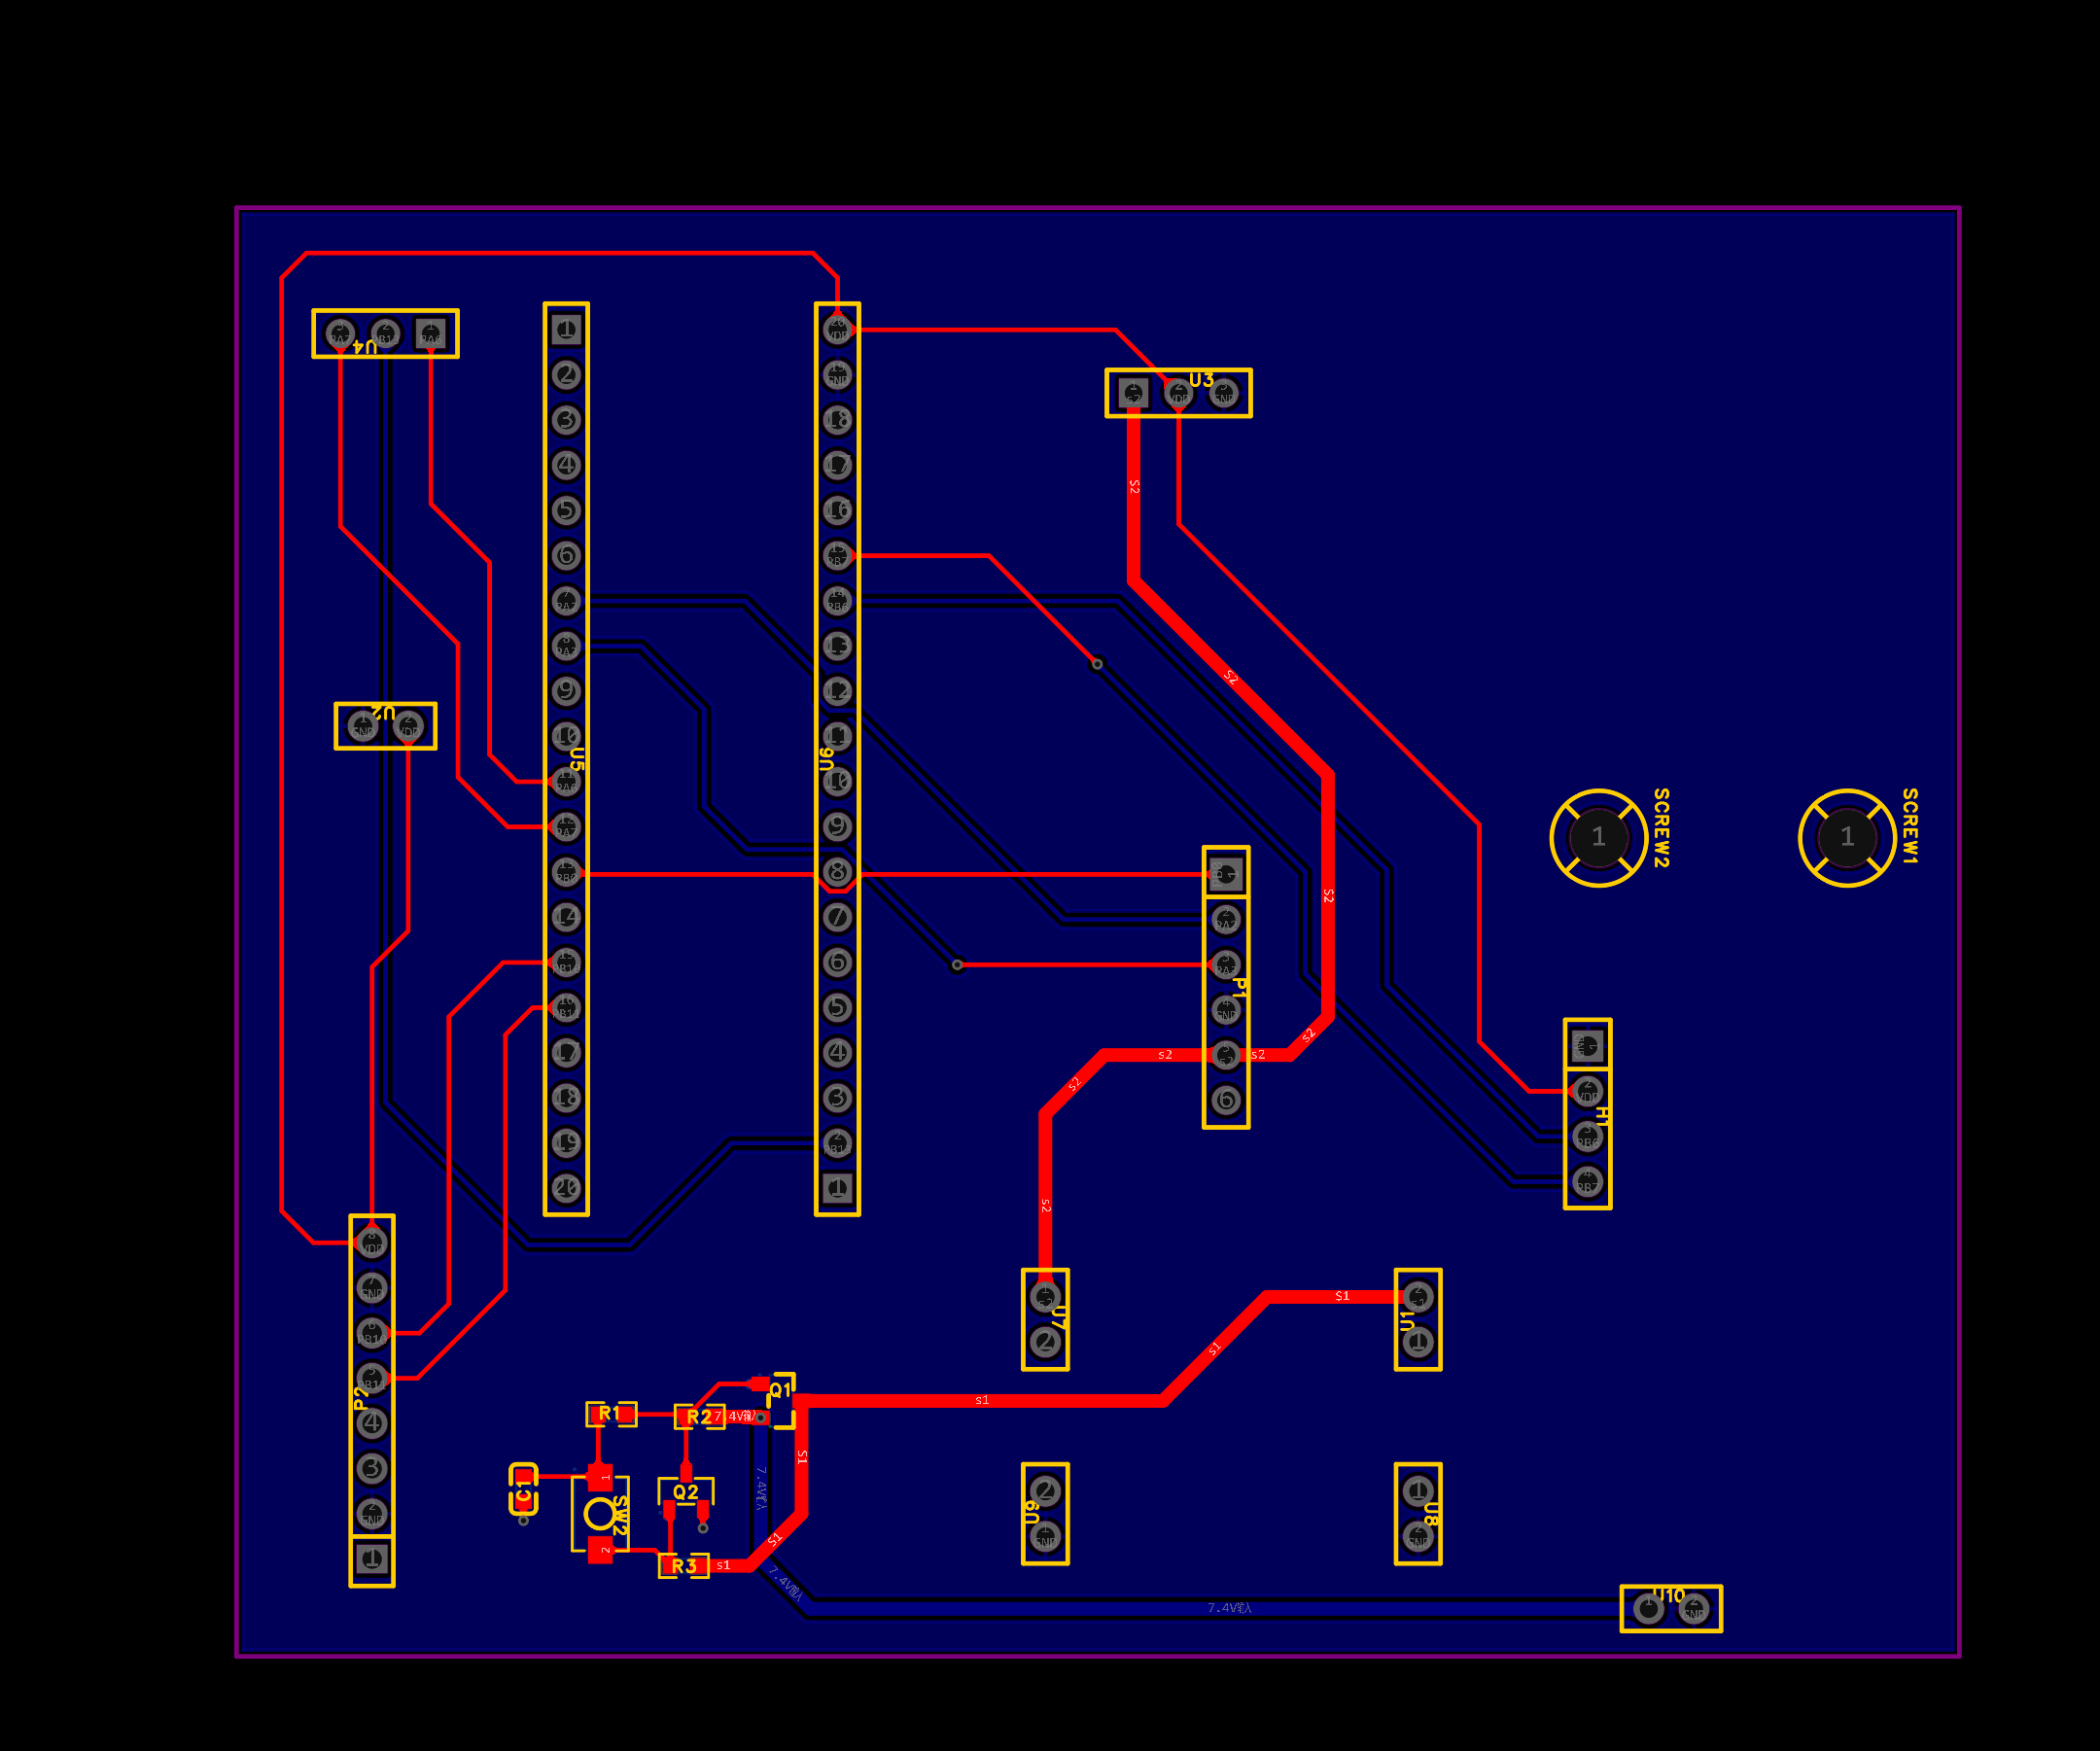
\includegraphics[width=0.9\textwidth]{figures/PCB终版.png}
    \caption{项目系统架构与功能模块总览（PCB终版布局，完整实现的硬件系统）}
    \label{fig:overview}
\end{figure}

\FloatBarrier